\documentclass{book}
\usepackage[UKenglish]{babel}
\usepackage{graphicx}
\usepackage{natbib}
\usepackage[colorlinks]{hyperref}
\usepackage[dvipsnames]{xcolor}
\usepackage{ amssymb, dsfont }
\usepackage{tikz}
\usepackage{dsfont}

\hypersetup{
  linkcolor  = Magenta,
  citecolor  = Aquamarine,
  urlcolor   = Periwinkle,
  linktoc    = page
}
\usepackage{algorithm}
\usepackage[noend]{algpseudocode}
\usepackage{amsmath,amssymb,bm}

\usepackage{enumitem}
\usepackage{subcaption}
\usepackage{wrapfig}
\usepackage{minted}  % Code embedding in document
\usepackage[none]{hyphenat}

\usepackage{mathtools}
\usepackage{verbatim}

\makeatletter
\newcommand\RedeclareMathOperator{%
  \@ifstar{\def\rmo@s{m}\rmo@redeclare}{\def\rmo@s{o}\rmo@redeclare}%
}
% this is taken from \renew@command
\newcommand\rmo@redeclare[2]{%
  \begingroup \escapechar\m@ne\xdef\@gtempa{{\string#1}}\endgroup
  \expandafter\@ifundefined\@gtempa
     {\@latex@error{\noexpand#1undefined}\@ehc}%
     \relax
  \expandafter\rmo@declmathop\rmo@s{#1}{#2}}
% This is just \@declmathop without \@ifdefinable
\newcommand\rmo@declmathop[3]{%
  \DeclareRobustCommand{#2}{\qopname\newmcodes@#1{#3}}%
}
\@onlypreamble\RedeclareMathOperator
\makeatother

\DeclareMathOperator{\E}{\mathbb{E}}
\DeclareMathOperator{\V}{\mathbb{V}}
\RedeclareMathOperator{\Pr}{\mathbb{P}}
\newcommand{\matr}[1]{\bm{#1}}     % ISO complying version
\newcommand{\vect}[1]{\bm{#1}}     % ISO complying version

\DeclarePairedDelimiter\ceil{\lceil}{\rceil}
\DeclarePairedDelimiter\floor{\lfloor}{\rfloor}

\DeclareMathOperator*{\argmax}{arg\,max}  % in your preamble
\DeclareMathOperator*{\argmin}{arg\,min}  % in your preamble 

\usepackage[nameinlink,noabbrev]{cleveref}
\newcommand*{\fullref}[1]{\hyperref[{#1}]{\Cref*{#1} -- \nameref*{#1}}}

\newcommand{\norm}[1]{\left\lVert#1\right\rVert}



\title{SP19 DL collaborative notes}
\author{
  The students of SP19 Deep Learning\\
  Editor: Alfredo Canziani\\
  NYU
}
\date{\today}

\begin{document}

\maketitle

\chapter*{Preface} \label{chp:preface}

This document aims to be a collection of lecture and laboratory notes, in an attempt to uniform the mathematical notation and gather all resources related to understand and master \emph{deep learning} in one, single location.

These notes are divided in five parts, which will constantly link to each other.
These are \fullref{prt:theory}, where the main topics will be introduced, \fullref{prt:practice}, where an intuition will be built about abstract concepts, \fullref{prt:coding}, where we'll see how to get our hands dirty with actual neural nets, on a computer, \fullref{prt:apps} where we'll encounter real life examples and applications, and \fullref{prt:papers} where short summary of the papers we've discussed will be nicely collected.
\chapter*{Instructions}

There are overall 42 hours of lectures.
For each hour there is a group of people assigned to summarise what happened in class \textbf{in roughly three pages}.
Each group is made of three students: two writers and a reviewer.

\section*{Writing directions}

Split your writing across the five parts of this document according to where it seems fit (see \nameref{chp:preface}).
Be consistent with the notation here specified.
\begin{itemize}[noitemsep,nolistsep]
\item Use \verb|\vect{}| and \verb|\matr{}| to decorate vectors and matrices respectively.
\item Start a new line \textbf{only and every time} you end a sentence with a period `.'; the \LaTeX\ engine will ignore this, but \verb|git| will love you.
\item Leave an empty line to start a new paragraph, and don't use the `\verb|\\|' break line (see \url{tex.stackexchange.com/a/225925/33287}).
\item Add date and group's authors name \textbf{as a comment}, after every \verb|\chapter|, \verb|\section|, and \verb|\subsection|.
\item The transposition symbol is obtained with \verb|^\top|. For example $(AB)^\top = B^\top A^\top$.
\end{itemize}

Feel free to create new chapters, sections, and subsections with corresponding labels \verb|\label{chp:}|, \verb|\label{sct:}|, and \verb|\label{ssc:}|.

\section*{Peer reviewing within groups}

Check for notation consistency, correctness, grammar, figure captioning, usage of \verb|\cref{}| instead of \verb|\ref{}|, \verb|\vect{}|, and \verb|\matr{}| to decorate vectors and matrices respectively, unnecessary use of bullet points or itemisations, missing references and use of links to papers PDF instead, usage of  $\Pr$, $\E$, and $\V$ for probability, expectation, and variance respectively using \verb|\Pr|, \verb|\E|, and \verb|\V|, \verb|\mid| for the conditional vertical bar, missing backslashes for $log, exp, max$ and any badly formatted functions, $\ast$ for convolutions, $\odot$ for element-wise multiplication, usage of \verb|\caption[Short caption]{Full caption}|, use of the correct transposition symbol obtained with \verb|^\top|, just to name a few.

\section*{Taking inspiration}

You can take inspiration from the work done by the students at NYU, who collectively wrote up the lecture notes in \href{https://www.overleaf.com/read/pchjywcxjkxn
}{this document} last year.
For example, you may reuse the following constructs, and others, at your convenience:
\[
\matr{X} = \begin{bmatrix}
    \rule[0.5mm]{0.8cm}{0.1mm} \; \vect{x}^{(1)} \; \rule[0.5mm]{0.8cm}{0.1mm} \\
    \rule[0.5mm]{0.8cm}{0.1mm} \; \vect{x}^{(2)} \; \rule[0.5mm]{0.8cm}{0.1mm} \\
    \vdots \\
    \rule[0.5mm]{0.8cm}{0.1mm} \; \vect{x}^{(m)} \; \rule[0.5mm]{0.8cm}{0.1mm} \\
\end{bmatrix}_{m \times n}
\matr{Y} = \begin{bmatrix}
    \rule[0.5mm]{0.8cm}{0.1mm} \; \vect{y}^{(1)} \; \rule[0.5mm]{0.8cm}{0.1mm} \\
    \rule[0.5mm]{0.8cm}{0.1mm} \; \vect{y}^{(2)} \; \rule[0.5mm]{0.8cm}{0.1mm} \\
    \vdots \\
    \rule[0.5mm]{0.8cm}{0.1mm} \; \vect{y}^{(m)} \; \rule[0.5mm]{0.8cm}{0.1mm} \\
\end{bmatrix}_{m \times K}
\]
\[
\hat{\matr{A}}\vect{x} =
\begin{bmatrix}
    \rule[0.5mm]{0.8cm}{0.1mm} \; \hat{\vect{a}}^{(1)} \; \rule[0.5mm]{0.8cm}{0.1mm} \\
    \rule[0.5mm]{0.8cm}{0.1mm} \; \hat{\vect{a}}^{(2)} \; \rule[0.5mm]{0.8cm}{0.1mm} \\
    \vdots \\
    \rule[0.5mm]{0.8cm}{0.1mm} \; \hat{\vect{a}}^{(m)} \; \rule[0.5mm]{0.8cm}{0.1mm} \\
\end{bmatrix}
\begin{pmatrix}
    \vrule height 0.6cm \\ \vect{x} \\ \vrule height 0.6cm
\end{pmatrix} =
\begin{pmatrix}
    \hat{\vect{a}}^{(1)} \vect{x} \\ \hat{\vect{a}}^{(2)} \vect{x} \\ \vdots \\ \hat{\vect{a}}^{(m)} \vect{x}
\end{pmatrix}_{m \times 1}
\]
\[
\matr{T}^{(1)}\vect{x} =
\begin{bmatrix}
    a_{1,1} & a_{1,2} & \dotsc & a_{1,k} & 0 & 0 & \dotsc & 0 \\
    0 & a_{1,1} & a_{1,2} & \dotsc & a_{1,k} & 0 & \dotsc & 0 \\
    0 & 0 & a_{1,1} & a_{1,2} & \dotsc & a_{1,k} & \dotsc & 0 \\
    \vdots & \vdots & \vdots & \ddots & \ddots & \ddots & \ddots & \vdots \\
    0 & \dotsc & 0 & 0 & a_{1,1} & a_{1,2} & \dotsc & a_{1,k}
\end{bmatrix}_{(n-k+1) \times n} =
\begin{pmatrix}
    \vect{a}^{(1)} \vect{x}_{1:1+k-1} \\ \vect{a}^{(1)} \vect{x}_{2:2+k-1} \\ \vdots \\ \vect{a}^{(1)}  \vect{x}_{n-k+1:n}
\end{pmatrix}_{(n-k+1) \times 1}
\]

Have fun!

\tableofcontents

%%%%%%%%%%%%%%%%%%%%%%%%%%%%%%%%%%%%%%%%%%
\part{Theory}\label{prt:theory}
%%%%%%%%%%%%%%%%%%%%%%%%%%%%%%%%%%%%%%%%%%
%%%%%%%%%%%%%%%%%%%%%%%%%%%%%%%%%%%%%%%%%%
\part{Practice}\label{prt:practice}
%%%%%%%%%%%%%%%%%%%%%%%%%%%%%%%%%%%%%%%%%%
\section{Tensor Transformations}
% Authors: Dustin Godevais , Reuben Juste, Yi Li,. 2/5/18.

The following sections summarize and visualize how you can transform data represented in matrix form. 
Input data can be defined as a matrix with the $i^{th}$ row corresponding to the $i^{th}$ data point and each additional columns representing a new dimension of the data.
$\matr{X}$ in the below examples is an input matrix with 1000 data points and two dimensions whose values are standard normally distributed. 
In the following figures, data points are colored according to their original $x_{N,1}$  dimension violet to yellow for negative to positive values.

\[
\matr{X} =
\begin{bmatrix}
    x_{1,1} & x_{1,2} \\
    x_{2,1} & x_{2,2} \\
    x_{3,1} & x_{3,2} \\
    \vdots & \vdots  \\
    x_{1000,1} & x_{1000,2}
\end{bmatrix}
\]

\begin{figure}[h]
\begin{center}
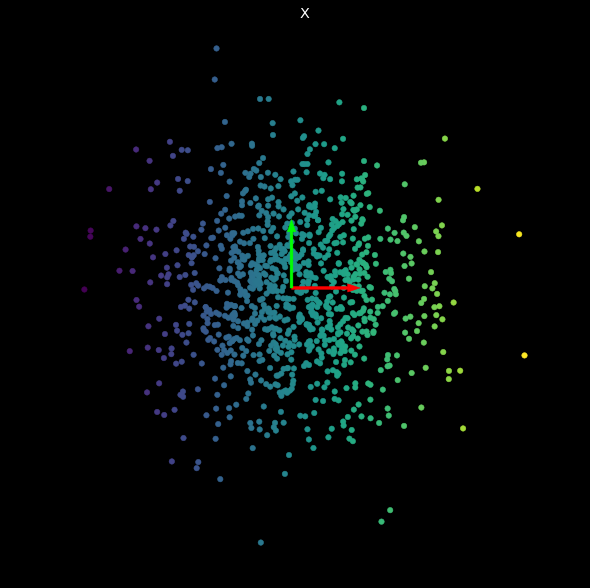
\includegraphics{students/SP19_DL_Lab_1_Notes/images/standardnormal.png}
\end{center} 
\caption{Original $\matr{X}$ Visualized}
\label{fig:mon}
\end{figure}

\subsection{Linear Transformations}
% Authors: Dustin Godevais , Reuben Juste, Yi Li,. 2/5/18.
There are several linear transformation that can be executed on $\matr{X}$ including:

\begin{itemize}
\tightlist
\item
Rotation (\(\matr{U}\))

\item
Scaling \((s_1, s_2)\)

\item
Reflection (\(\matr{V}\))
\item
Shearing
\item
Translation
\end{itemize}

The product of the first three form weights as shown below.

\[
\matr{W} = \matr{U}
\begin{bmatrix}
    s_1 & 0 \\
    0 & s_2 
\end{bmatrix}
\matr{V}^T
\]


\subsubsection{Rotation}
During rotation, each point is rotated about the origin by the indicated angle. 
The below equation populates $\matr{U}$ based on rotating points by \(\theta\) counter-clockwise.

\[
\matr{U} = 
\begin{bmatrix}
    cos(\theta) & sin(\theta)\\
    sin(\theta) & -cos(\theta)
\end{bmatrix}
\]

Keeping scaling and reflection constant, the below figure shows a set up points with different  \(\theta\)s .

\begin{figure}[h!]
\begin{center}
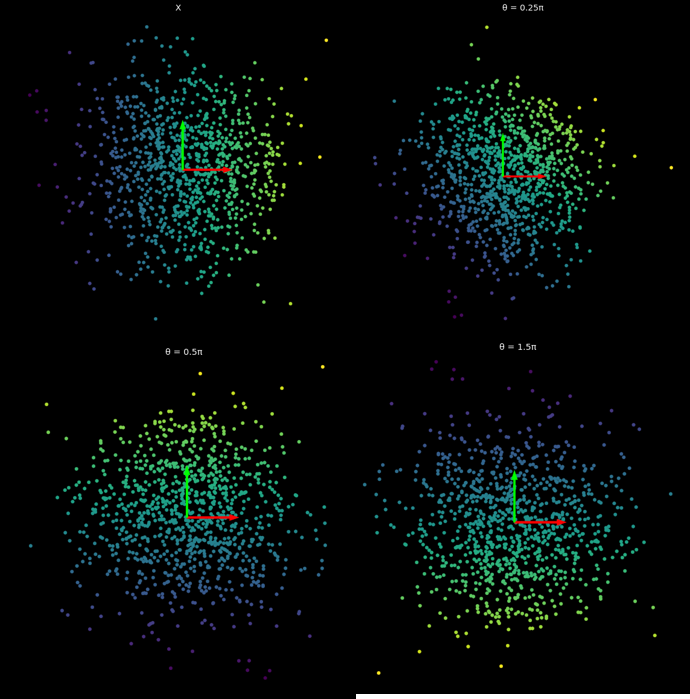
\includegraphics{students/SP19_DL_Lab_1_Notes/images/Rotation.png}
\end{center} 
\caption{Rotation Visualized}
\label{fig:mon}
\end{figure}
\FloatBarrier


\subsubsection{Scaling}
Scaling the points expands or contracts the points about the origin. 
This controlled separately for each dimension by \(s_1\) and \(s_2\) .

\begin{figure}[h!]
\begin{center}
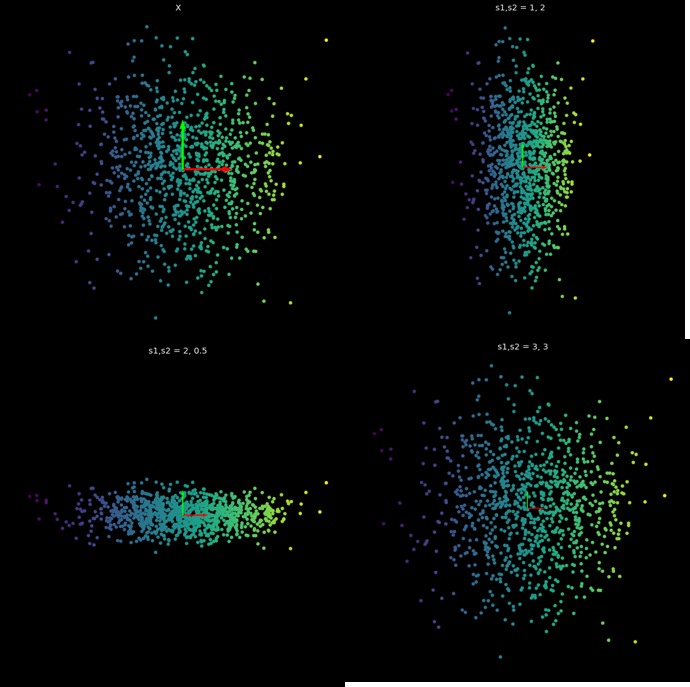
\includegraphics{students/SP19_DL_Lab_1_Notes/images/Scaling.png}
\caption{Scaling Visualized}
\label{fig:mon}
\end{center} 
\end{figure}
\FloatBarrier


\subsubsection{Reflection}
Reflecting points projects them on the other side of a defined line that crosses the origin. 
The line that goes from the original point to the projected point is perpendicular to the defined line, and the intersection to the defined line is the midpoint.


\begin{figure}[h!]
\begin{center}

\includegraphics{students/SP19_DL_Lab_1_Notes/images/reflection_example.png}
\end{center} 
\caption{Reflection Defined}
\label{fig:mon}
\end{figure}
\FloatBarrier


\(\matr{V}\) can be defined by

\[
\matr{V} = 
\begin{bmatrix}
    cos(2\theta) & sin(2\theta)\\
    sin(2\theta) & -cos(2\theta)
\end{bmatrix}
\]

Where the defined line is \(x_2 = tan(\theta) x_1 \)

\begin{figure}[h!]
\begin{center}
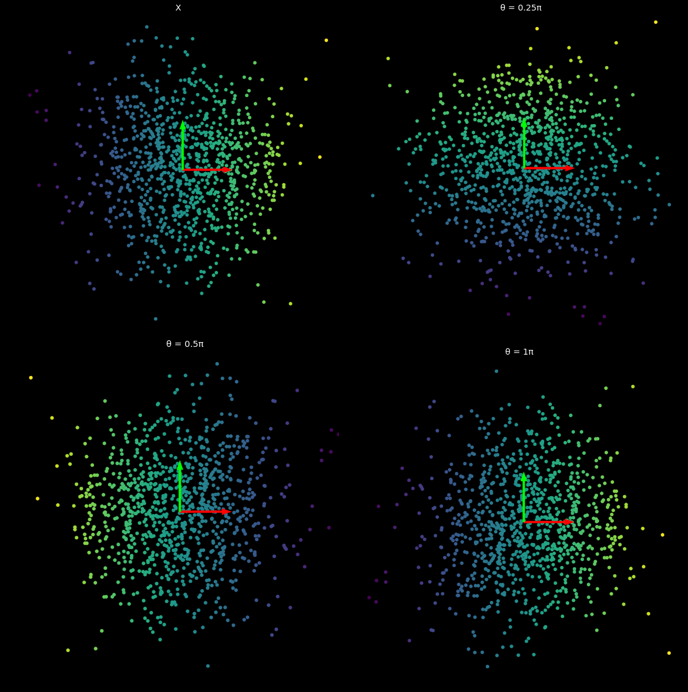
\includegraphics{students/SP19_DL_Lab_1_Notes/images/Reflection.png}
\end{center} 
\caption{Reflection Visualized}
\label{fig:mon}
\end{figure}
\FloatBarrier

\subsubsection{Shearing}
Shearing points, which is separate from the weight calculation, shifting points in one dimension proportional to their value in the other dimension.

\(\matr{Y} = \matr{X}  \begin{bmatrix}
    1 & k\\
    0 & 1
\end{bmatrix} \) 
Shift points on the \(x_1\) dimension proportional to the \(x_2\) dimension

\(\matr{Y} = \matr{X}  \begin{bmatrix}
    1 & 0\\
    k & 1
\end{bmatrix} \)
Shift points on the \(x_2\) dimension proportional to the \(x_1\) dimension

\begin{figure}[h!]
\begin{center}
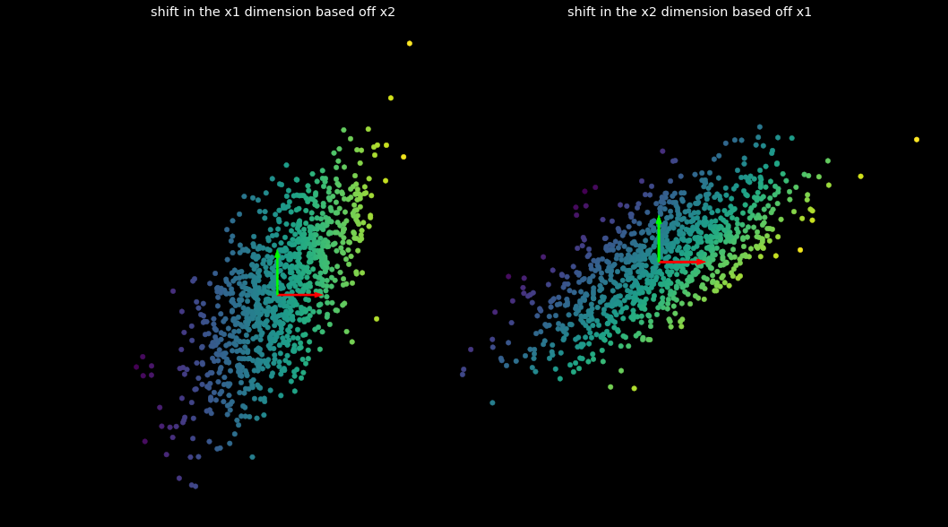
\includegraphics{students/SP19_DL_Lab_1_Notes/images/shear.png}
\end{center} 
\caption{Shear Visualized}
\label{fig:mon}
\end{figure}
\FloatBarrier

\subsubsection{Translation}
The translation of points, which is separate from the weight calculations moves them uniforming in the direction indicated.

\[ \matr{Y} = \matr{X} 
+ \begin{bmatrix}
    1 & 1 \\
    1 & 1 \\
    1 & 1 \\
    \vdots & \vdots  \\
    1 & 1
\end{bmatrix}
\begin{bmatrix}
    t_1 & 0\\
    0 & t_2
\end{bmatrix} \] 
(Shift points left or right by \(t_1\) and up or down by  \(t_2\) dimension)

\begin{figure}[h!]
\begin{center}
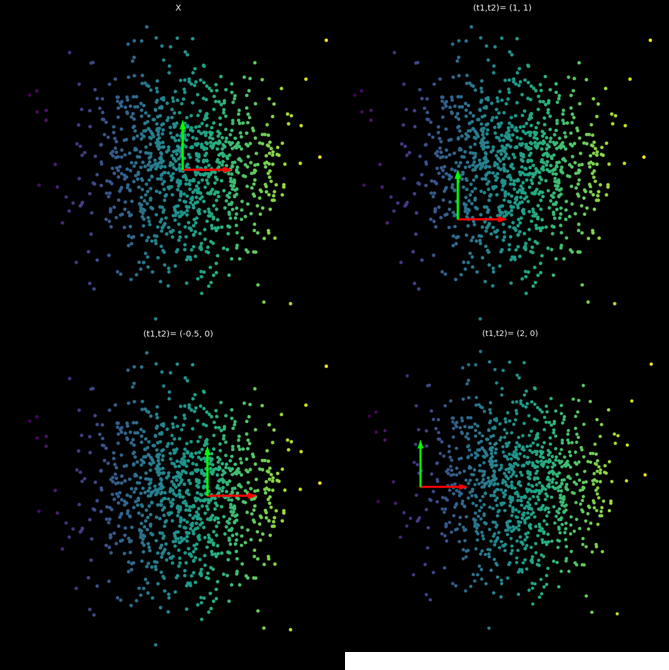
\includegraphics{students/SP19_DL_Lab_1_Notes/images/translation.png}
\end{center} 
\caption{Translation Visualized}
\label{fig:mon}
\end{figure}
\FloatBarrier

\subsection{Non-Linear Transformations}
% Authors: Dustin Godevais , Reuben Juste, Yi Li,. 2/5/18.
Linear transformations are capable of altering data in many different ways, but linear transformations cannot curve data. 
That is where non-linear transformations come in. There are several types of non-linear transformations such as:

\begin{itemize}
\tightlist
\item
Rectified linear unit (Relu) - \(y= x_1\) if \(x_1 > 0\) else  0 
\item
Polynomial- \(y = x_1^2\) or \(y = x_1 x_2\)

\item
Step - \(y = 1 \) if \(x > 0 \) else 0 

\end{itemize}

One of the most common non-linear transformations is Tanh, which in the context of 2D Tensors can be applied as below:
\[f(x) = tanh(
\begin{bmatrix}
s & 0\\
0 & s
\end{bmatrix}
x)\]

This function first stretches out the points using scalar s via \hyperref[subsubsec:Scaling]{scaling}, then tanh squashes the points into a square.
The larger s is, the more points end up in the square.

\begin{figure}[h!]
\begin{center}
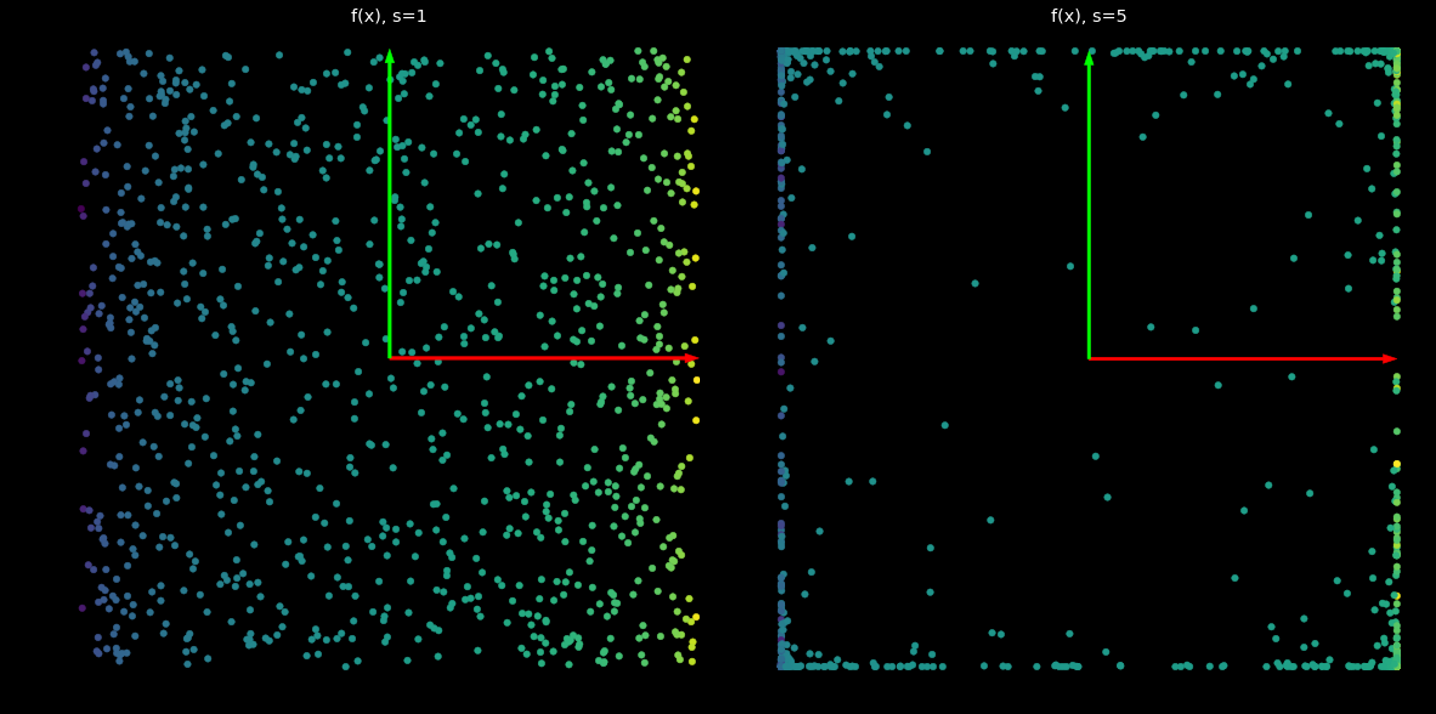
\includegraphics{students/SP19_DL_Lab_1_Notes/images/tanh.png}
\end{center} 
\caption{Tanh in Isolation}
\label{fig:mon}
\end{figure}
\FloatBarrier

Tanh can create curved surfaces when it is sandwiched in-between two linear transformations in a three layer neural network.

\begin{figure}[h!]
\begin{center}
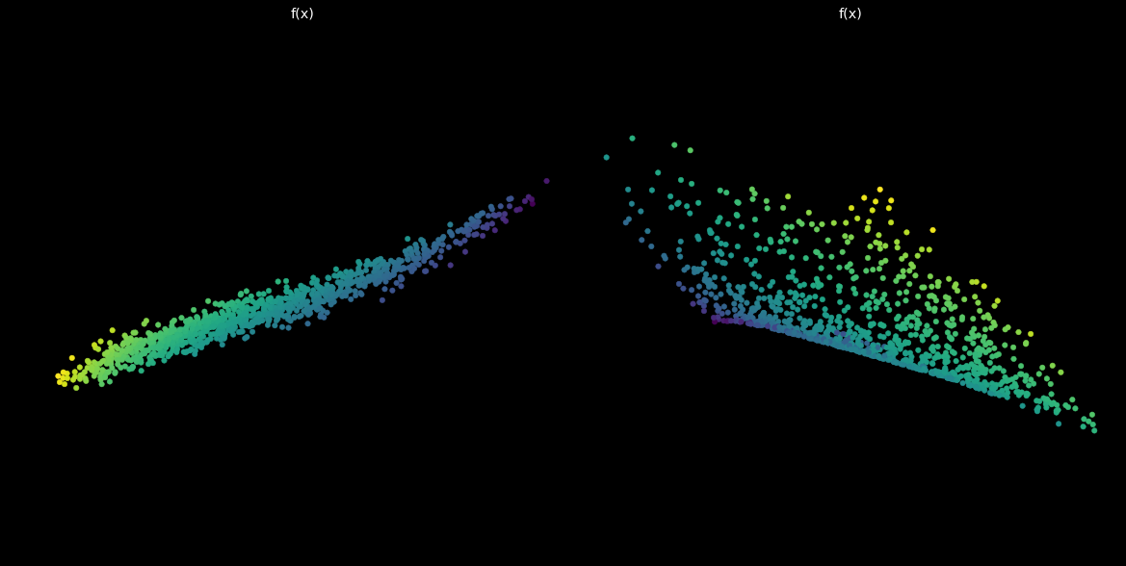
\includegraphics{students/SP19_DL_Lab_1_Notes/images/tanh_sandwich.png}
\end{center} 
\caption{Tanh In-Between Two Linear Layers}
\label{fig:mon}
\end{figure}
\FloatBarrier

%%%%%%%%%%%%%%%%%%%%%%%%%%%%%%%%%%%%%%%%%%
\part{Coding}\label{prt:coding}
%%%%%%%%%%%%%%%%%%%%%%%%%%%%%%%%%%%%%%%%%%

\section{Introduction to \emph{PyTorch} and \texttt{Tensor}s}
% Authors: Dustin Godevais , Reuben Juste, Yi Li,. 2/5/18.
    \subsection{What is \emph{PyTorch}?}\label{what-is-pytorch}
    % Authors: Dustin Godevais , Reuben Juste, Yi Li,. 2/5/18.
    \emph{PyTorch} is a Python based scientific computing package targeting on two sets of audiences:

   
\begin{itemize}
\tightlist
\item
  Tensorial library that uses the power of GPUs
\item
  A deep learning research platform that provides maximum flexibility
  and speed
\end{itemize}

    
     \begin{Verbatim}[commandchars=\\\{\}]
{\color{incolor}In [{\color{incolor}1}]:} \PY{k+kn}{import} \PY{n+nn}{torch}
\end{Verbatim}

    \subsection{Getting help in Jupyter}\label{getting-help-in-jupyter}
    % Authors: Dustin Godevais , Reuben Juste, Yi Li,. 2/5/18.

    
%\subsection*{Jupyter Tips}
    \href{https://jupyter.org/}{Jupyter Notebook} is a common Integrated Development Environment (IDE) for deep learning. There are a few commands specific to Jupyter Notebook that are helpful for coding.   
        \subsubsection{Using tab}
        Tab will list all available functions, while shift + tab will open the documentation.

        \subsubsection{Using ?}
        \begin{Verbatim}[commandchars=\\\{\}]
{\color{incolor}In [{\color{incolor}2}]:} \PY{c+c1}{\PYZsh{} Open the documentation, same as \PYZlt{}shift\PYZgt{} + \PYZlt{}tab\PYZgt{} on \PYZsq{}torch.nn.Module()\PYZsq{}}
         torch.nn.Module\PY{o}{?}
\end{Verbatim}


    \begin{Verbatim}[commandchars=\\\{\}]
{\color{incolor}In [{\color{incolor}3}]:} \PY{c+c1}{\PYZsh{} See the source code of all functions being executed in the Module}
         torch.nn.Module\PY{o}{??}
\end{Verbatim}
        
\subsubsection{Dropping to Bash}
\begin{Verbatim}[commandchars=\\\{\}]
{\color{incolor}In [{\color{incolor}4}]:} \PY{c+c1}{\PYZsh{} List all the files in the current directory}
         \PY{o}{!}ls \PYZhy{}lh 
\end{Verbatim}

\begin{Verbatim}[commandchars=\\\{\}]
{\color{incolor}In [{\color{incolor}5}]:} \PY{c+c1}{\PYZsh{} Getting some general help}
         \PY{o}{\PYZpc{}}\PY{k}{magic} 
\end{Verbatim}

\subsection{Tensors}\label{tensors}   
% Authors: Dustin Godevais , Reuben Juste, Yi Li,. 2/5/18.
A tensor is a n-dimensional array, \emph{PyTorch} provides functions for operating on Tensors like numpy does for arrays.
\begin{Verbatim}[commandchars=\\\{\}]
{\color{incolor}In [{\color{incolor}6}]:} \PY{c+c1}{\PYZsh{} Generate a tensor of size 2x3x4}
         \PY{n}{t} \PY{o}{=} \PY{n}{torch}\PY{o}{.}\PY{n}{Tensor}\PY{p}{(}\PY{l+m+mi}{2}\PY{p}{,} \PY{l+m+mi}{3}\PY{p}{,} \PY{l+m+mi}{4}\PY{p}{)}
         \PY{n+nb}{type}\PY{p}{(}\PY{n}{t}\PY{p}{)} 
\end{Verbatim}


\begin{Verbatim}[commandchars=\\\{\}]
{\color{outcolor}Out[{\color{outcolor}6}]:} torch.Tensor
\end{Verbatim}
            
\begin{Verbatim}[commandchars=\\\{\}]
{\color{incolor}In [{\color{incolor}7}]:} \PY{c+c1}{\PYZsh{} Get the size of the tensor}
         \PY{n}{t}\PY{o}{.}\PY{n}{size}\PY{p}{(}\PY{p}{)} 
\end{Verbatim}


\begin{Verbatim}[commandchars=\\\{\}]
{\color{outcolor}Out[{\color{outcolor}7}]:} torch.Size([2, 3, 4])
\end{Verbatim}
            
\begin{Verbatim}[commandchars=\\\{\}]
{\color{incolor}In [{\color{incolor}8}]:} \PY{c+c1}{\PYZsh{} Get the dimension of the tensor, for example, 1 for vectors, 2 for matrices}
         \PY{n}{t}\PY{o}{.}\PY{n}{dim}\PY{p}{(}\PY{p}{)} 
\end{Verbatim}


\begin{Verbatim}[commandchars=\\\{\}]
{\color{outcolor}Out[{\color{outcolor}8}]:} 3
\end{Verbatim}
            
\begin{Verbatim}[commandchars=\\\{\}]
{\color{incolor}In [{\color{incolor}9}]:} \PY{c+c1}{\PYZsh{} Total number of elements in the tensor}
         \PY{n}{t}\PY{o}{.}\PY{n}{numel}\PY{p}{(}\PY{p}{)} 
\end{Verbatim}


\begin{Verbatim}[commandchars=\\\{\}]
{\color{outcolor}Out[{\color{outcolor}9}]:} 24
\end{Verbatim}
 
Note: Mind the underscore! 
Any operation that mutates a tensor in-place is post-fixed with an underscore. 
The in-place replacement will change the object. It is encouraged to perform operations in-place to optimize usage of memory.
            
\begin{Verbatim}[commandchars=\\\{\}]
{\color{incolor}In [{\color{incolor}10}]:} 
         \PY{n}{t}\PY{o}{.}\PY{n}{random\PYZus{}}\PY{p}{(}\PY{l+m+mi}{10}\PY{p}{)} 
\end{Verbatim}


\begin{Verbatim}[commandchars=\\\{\}]
{\color{outcolor}Out[{\color{outcolor}10}]:} tensor([[[4., 6., 2., 4.],
                  [8., 2., 6., 9.],
                  [1., 4., 9., 9.]],
         
                 [[8., 5., 5., 5.],
                  [4., 1., 1., 7.],
                  [4., 4., 6., 9.]]])
\end{Verbatim}
            
\begin{Verbatim}[commandchars=\\\{\}]
{\color{incolor}In [{\color{incolor}11}]:} \PY{n}{r} \PY{o}{=} \PY{n}{torch}\PY{o}{.}\PY{n}{Tensor}\PY{p}{(}\PY{n}{t}\PY{p}{)}
         \PY{c+c1}{\PYZsh{} This resizes the tensor permanently}
         \PY{n}{r}\PY{o}{.}\PY{n}{resize\PYZus{}}\PY{p}{(}\PY{l+m+mi}{3}\PY{p}{,} \PY{l+m+mi}{8}\PY{p}{)}  
         \PY{n}{r}
\end{Verbatim}


\begin{Verbatim}[commandchars=\\\{\}]
{\color{outcolor}Out[{\color{outcolor}11}]:} tensor([[4., 6., 2., 4., 8., 2., 6., 9.],
                 [1., 4., 9., 9., 8., 5., 5., 5.],
                 [4., 1., 1., 7., 4., 4., 6., 9.]])
\end{Verbatim}
            
\begin{Verbatim}[commandchars=\\\{\}]
{\color{incolor}In [{\color{incolor}12}]:} \PY{c+c1}{\PYZsh{} Replace all element in r with 0\PYZsq{}s}
         \PY{n}{r}\PY{o}{.}\PY{n}{zero\PYZus{}}\PY{p}{(}\PY{p}{)} 
\end{Verbatim}


\begin{Verbatim}[commandchars=\\\{\}]
{\color{outcolor}Out[{\color{outcolor}12}]:} tensor([[0., 0., 0., 0., 0., 0., 0., 0.],
                 [0., 0., 0., 0., 0., 0., 0., 0.],
                 [0., 0., 0., 0., 0., 0., 0., 0.]])
\end{Verbatim}
            
\begin{Verbatim}[commandchars=\\\{\}]
{\color{incolor}In [{\color{incolor}13}]:} \PY{n}{t}
\end{Verbatim}


\begin{Verbatim}[commandchars=\\\{\}]
{\color{outcolor}Out[{\color{outcolor}13}]:} tensor([[[0., 0., 0., 0.],
                  [0., 0., 0., 0.],
                  [0., 0., 0., 0.]],
         
                 [[0., 0., 0., 0.],
                  [0., 0., 0., 0.],
                  [0., 0., 0., 0.]]])
\end{Verbatim}
         
            
\begin{Verbatim}[commandchars=\\\{\}]
{\color{incolor}In [{\color{incolor}14}]:} \PY{c+c1}{\PYZsh{} Make a copy of r rather than replace r. }
         \PY{n}{s} \PY{o}{=} \PY{n}{r}\PY{o}{.}\PY{n}{clone}\PY{p}{(}\PY{p}{)} 
\end{Verbatim}
 Q: Why don\PYZsq{}t we always do this? \\
 A: It's time-consuming due to memory allocation, especially when we are training a neural network.  


\begin{Verbatim}[commandchars=\\\{\}]
{\color{incolor}In [{\color{incolor}15}]:} \PY{c+c1}{\PYZsh{} In\PYZhy{}place fill of 1\PYZsq{}s}
         \PY{n}{s}\PY{o}{.}\PY{n}{fill\PYZus{}}\PY{p}{(}\PY{l+m+mi}{1}\PY{p}{)} 
         \PY{n}{s}
\end{Verbatim}


\begin{Verbatim}[commandchars=\\\{\}]
{\color{outcolor}Out[{\color{outcolor}15}]:} tensor([[1., 1., 1., 1., 1., 1., 1., 1.],
                 [1., 1., 1., 1., 1., 1., 1., 1.],
                 [1., 1., 1., 1., 1., 1., 1., 1.]])
\end{Verbatim}
            
\begin{Verbatim}[commandchars=\\\{\}]
{\color{incolor}In [{\color{incolor}16}]:} \PY{c+c1}{\PYZsh{} Because we cloned r, even though we did an in\PYZhy{}place operation, this doesn\PYZsq{}t affect r}
         \PY{n}{r} 
\end{Verbatim}


\begin{Verbatim}[commandchars=\\\{\}]
{\color{outcolor}Out[{\color{outcolor}16}]:} tensor([[0., 0., 0., 0., 0., 0., 0., 0.],
                 [0., 0., 0., 0., 0., 0., 0., 0.],
                 [0., 0., 0., 0., 0., 0., 0., 0.]])
\end{Verbatim}
          

\subsubsection{Vectors: 1D Tensor}
\begin{Verbatim}[commandchars=\\\{\}]
{\color{incolor}In [{\color{incolor}17}]:} \PY{n}{v} \PY{o}{=} \PY{n}{torch}\PY{o}{.}\PY{n}{Tensor}\PY{p}{(}\PY{p}{[}\PY{l+m+mi}{1}\PY{p}{,} \PY{l+m+mi}{2}\PY{p}{,} \PY{l+m+mi}{3}\PY{p}{,} \PY{l+m+mi}{4}\PY{p}{]}\PY{p}{)}
         \PY{n}{w} \PY{o}{=} \PY{n}{torch}\PY{o}{.}\PY{n}{Tensor}\PY{p}{(}\PY{p}{[}\PY{l+m+mi}{1}\PY{p}{,} \PY{l+m+mi}{0}\PY{p}{,} \PY{l+m+mi}{2}\PY{p}{,} \PY{l+m+mi}{0}\PY{p}{]}\PY{p}{)}
         \PY{c+c1}{\PYZsh{} Element\PYZhy{}wise multiplication}
         \PY{n}{v} \PY{o}{*} \PY{n}{w} 
\end{Verbatim}


\begin{Verbatim}[commandchars=\\\{\}]
{\color{outcolor}Out[{\color{outcolor}17}]:} tensor([1., 0., 6., 0.])
\end{Verbatim}
            
\begin{Verbatim}[commandchars=\\\{\}]
{\color{incolor}In [{\color{incolor}18}]:} \PY{c+c1}{\PYZsh{} Scalar product: 1*1 + 2*0 + 3*2 + 4*0}
         \PY{n}{v} \PY{o}{@} \PY{n}{w} 
\end{Verbatim}


\begin{Verbatim}[commandchars=\\\{\}]
{\color{outcolor}Out[{\color{outcolor}18}]:} tensor(7.)
\end{Verbatim}
            
\begin{Verbatim}[commandchars=\\\{\}]
{\color{incolor}In [{\color{incolor}19}]:} \PY{n}{x} \PY{o}{=} \PY{n}{torch}\PY{o}{.}\PY{n}{Tensor}\PY{p}{(}\PY{l+m+mi}{5}\PY{p}{)}\PY{o}{.}\PY{n}{random\PYZus{}}\PY{p}{(}\PY{l+m+mi}{10}\PY{p}{)}
         \PY{n}{x}
\end{Verbatim}


\begin{Verbatim}[commandchars=\\\{\}]
{\color{outcolor}Out[{\color{outcolor}19}]:} tensor([6., 0., 5., 9., 7.])
\end{Verbatim}
            
   

\begin{Verbatim}[commandchars=\\\{\}]
{\color{incolor}In [{\color{incolor}20}]:} \PY{c+c1}{\PYZsh{} Extract sub\PYZhy{}Tensor [from:to)}
         \PY{n}{x}\PY{p}{[}\PY{l+m+mi}{1}\PY{p}{:}\PY{l+m+mi}{2} \PY{o}{+} \PY{l+m+mi}{1}\PY{p}{]} 
\end{Verbatim}


\begin{Verbatim}[commandchars=\\\{\}]
{\color{outcolor}Out[{\color{outcolor}20}]:} tensor([0., 5.])
\end{Verbatim}
       
Note: torch.arange gives only integers. Use torch.arange(1, 4 + 1, dtype = torch.float) to generate float numbers.      
            
\begin{Verbatim}[commandchars=\\\{\}]
{\color{incolor}In [{\color{incolor}21}]:} \PY{c+c1}{\PYZsh{} Create a tensor with integers ranging from 1 to 5, excluding 5}
         \PY{n}{v} \PY{o}{=} \PY{n}{torch}\PY{o}{.}\PY{n}{arange}\PY{p}{(}\PY{l+m+mi}{1}\PY{p}{,} \PY{l+m+mi}{4} \PY{o}{+} \PY{l+m+mi}{1}\PY{p}{)} 
         \PY{n}{v} 
\end{Verbatim}


\begin{Verbatim}[commandchars=\\\{\}]
{\color{outcolor}Out[{\color{outcolor}21}]:} tensor([1, 2, 3, 4])
\end{Verbatim}
\subsubsection{Matrices: 2D Tensor}
\begin{Verbatim}[commandchars=\\\{\}]
{\color{incolor}In [{\color{incolor}22}]:} \PY{c+c1}{\PYZsh{} Create a 2x4 tensor}
         \PY{n}{m} \PY{o}{=} \PY{n}{torch}\PY{o}{.}\PY{n}{Tensor}\PY{p}{(}\PY{p}{[}\PY{p}{[}\PY{l+m+mi}{2}\PY{p}{,} \PY{l+m+mi}{5}\PY{p}{,} \PY{l+m+mi}{3}\PY{p}{,} \PY{l+m+mi}{7}\PY{p}{]}\PY{p}{,}
                           \PY{p}{[}\PY{l+m+mi}{4}\PY{p}{,} \PY{l+m+mi}{2}\PY{p}{,} \PY{l+m+mi}{1}\PY{p}{,} \PY{l+m+mi}{9}\PY{p}{]}\PY{p}{]}\PY{p}{)} 
\end{Verbatim}
            
\begin{Verbatim}[commandchars=\\\{\}]
{\color{incolor}In [{\color{incolor}23}]:} \PY{c+c1}{\PYZsh{} Indexing column 0, row 2, it returns a 0\PYZhy{}dimensional tensor, which is a scalar. Or m[0,2]}
          \PY{n}{m}\PY{p}{[}\PY{l+m+mi}{0}\PY{p}{]}\PY{p}{[}\PY{l+m+mi}{2}\PY{p}{]} 
\end{Verbatim}


\begin{Verbatim}[commandchars=\\\{\}]
{\color{outcolor}Out[{\color{outcolor}23}]:} tensor(3.)
\end{Verbatim}
            
\begin{Verbatim}[commandchars=\\\{\}]
{\color{incolor}In [{\color{incolor}24}]:} \PY{c+c1}{\PYZsh{} Extract the single value in the scalar}
          \PY{n}{m}\PY{p}{[}\PY{l+m+mi}{0}\PY{p}{,}\PY{l+m+mi}{2}\PY{p}{]}\PY{o}{.}\PY{n}{item}\PY{p}{(}\PY{p}{)} 
\end{Verbatim}
Q: Why won't we extract value always? \\
A: A tensor will remember who is the parent, so we need to use tensor rather than just the scalar number when we perform back propagation during training a neural network.

\begin{Verbatim}[commandchars=\\\{\}]
{\color{outcolor}Out[{\color{outcolor}24}]:} 3.0
\end{Verbatim}
            
\begin{Verbatim}[commandchars=\\\{\}]
{\color{incolor}In [{\color{incolor}25}]:} \PY{c+c1}{\PYZsh{} Indexing column 1, all rows (returns size 2)}
          \PY{n}{m}\PY{p}{[}\PY{p}{:}\PY{p}{,} \PY{l+m+mi}{1}\PY{p}{]} 
\end{Verbatim}


\begin{Verbatim}[commandchars=\\\{\}]
{\color{outcolor}Out[{\color{outcolor}25}]:} tensor([5., 2.])
\end{Verbatim}
            
\begin{Verbatim}[commandchars=\\\{\}]
{\color{incolor}In [{\color{incolor}26}]:} \PY{c+c1}{\PYZsh{} Add one more bracket inside will add an extra dimension, now it\PYZsq{}s a 2 * 1 matrix }
          \PY{n}{m}\PY{p}{[}\PY{p}{:}\PY{p}{,} \PY{p}{[}\PY{l+m+mi}{1}\PY{p}{]}\PY{p}{]} 
\end{Verbatim}


\begin{Verbatim}[commandchars=\\\{\}]
{\color{outcolor}Out[{\color{outcolor}26}]:} tensor([[5.],
                  [2.]])
\end{Verbatim}

            
\begin{Verbatim}[commandchars=\\\{\}]
{\color{incolor}In [{\color{incolor}27}]:} \PY{c+c1}{\PYZsh{} Same as m.transpose(0, 1)}
          \PY{n}{m}\PY{o}{.}\PY{n}{t}\PY{p}{(}\PY{p}{)} 
\end{Verbatim}
Note: We can specify dimensions dimensions we want to swap using m.transpose(c1,c2) when we have many dimensions.

\begin{Verbatim}[commandchars=\\\{\}]
{\color{outcolor}Out[{\color{outcolor}27}]:} tensor([[2., 4.],
                  [5., 2.],
                  [3., 1.],
                  [7., 9.]])
\end{Verbatim}
            
\begin{Verbatim}[commandchars=\\\{\}]
{\color{incolor}In [{\color{incolor}28}]:} \PY{c+c1}{\PYZsh{} Create tensor from 3 to 8, with each having a space of 1}
          \PY{n}{torch}\PY{o}{.}\PY{n}{arange}\PY{p}{(}\PY{l+m+mf}{3.}\PY{p}{,} \PY{l+m+mi}{8} \PY{o}{+} \PY{l+m+mi}{1}\PY{p}{)} 
\end{Verbatim}


\begin{Verbatim}[commandchars=\\\{\}]
{\color{outcolor}Out[{\color{outcolor}28}]:} tensor([3., 4., 5., 6., 7., 8.])
\end{Verbatim}
            
\begin{Verbatim}[commandchars=\\\{\}]
{\color{incolor}In [{\color{incolor}29}]:} \PY{c+c1}{\PYZsh{} returns a 1D tensor of steps equally spaced points between start=3, end=8 and steps=20}
          \PY{n}{torch}\PY{o}{.}\PY{n}{linspace}\PY{p}{(}\PY{l+m+mi}{3}\PY{p}{,} \PY{l+m+mi}{8}\PY{p}{,} \PY{l+m+mi}{20}\PY{p}{)}\PY{o}{.}\PY{n}{view}\PY{p}{(}\PY{l+m+mi}{1}\PY{p}{,} \PY{o}{\PYZhy{}}\PY{l+m+mi}{1}\PY{p}{)} 
\end{Verbatim}


\begin{Verbatim}[commandchars=\\\{\}]
{\color{outcolor}Out[{\color{outcolor}29}]:} tensor([[3.0000, 3.2632, 3.5263, 3.7895, 4.0526, 4.3158, 4.5789, 4.8421, 5.1053,
                   5.3684, 5.6316, 5.8947, 6.1579, 6.4211, 6.6842, 6.9474, 7.2105, 7.4737,
                   7.7368, 8.0000]])
\end{Verbatim}
            
\begin{Verbatim}[commandchars=\\\{\}]
{\color{incolor}In [{\color{incolor}30}]:} \PY{c+c1}{\PYZsh{} Create a tensor filled with 0\PYZsq{}s torch.ones() will create a tensor filled with 1\PYZsq{}s.}
          \PY{n}{torch}\PY{o}{.}\PY{n}{zeros}\PY{p}{(}\PY{l+m+mi}{3}\PY{p}{,} \PY{l+m+mi}{5}\PY{p}{)} 
\end{Verbatim}


\begin{Verbatim}[commandchars=\\\{\}]
{\color{outcolor}Out[{\color{outcolor}30}]:} tensor([[0., 0., 0., 0., 0.],
                  [0., 0., 0., 0., 0.],
                  [0., 0., 0., 0., 0.]])
\end{Verbatim}
            
\begin{Verbatim}[commandchars=\\\{\}]
{\color{incolor}In [{\color{incolor}31}]:} \PY{c+c1}{\PYZsh{} Create a tensor with the diagonal filled with 1}
          \PY{n}{torch}\PY{o}{.}\PY{n}{eye}\PY{p}{(}\PY{l+m+mi}{3}\PY{p}{)}
\end{Verbatim}


\begin{Verbatim}[commandchars=\\\{\}]
{\color{outcolor}Out[{\color{outcolor}31}]:} tensor([[1., 0., 0.],
                  [0., 1., 0.],
                  [0., 0., 1.]])
\end{Verbatim}
\subsubsection{Images: 3D Tensor}
Q: Why would we use 4D Tensors while training convolutional neural networks?\\
A: Images are 3D Tensors with dimensions channels, height, and width. We will use a stack of multiple images to form a 4-dimensional tensor.


\section{References}
% Authors: Dustin Godevais , Reuben Juste, Yi Li,. 2/5/18.
\begin{itemize}
\tightlist
\item
\href{https://www.technologyuk.net/mathematics/algebra/matrices-as-transformations.shtml}{https://www.technologyuk.net/mathematics/algebra/matrices-as-transformations.shtml}
\item
\href{https://github.com/Atcold/pytorch-Deep-Learning-Minicourse/blob/master/01-tensor_tutorial.ipynb}{https://github.com/Atcold/pytorch-Deep-Learning-Minicourse/blob/master/01-tensor_tutorial.ipynb}
\item
\href{https://github.com/Atcold/pytorch-Deep-Learning-Minicourse/blob/master/02-space_stretching.ipynb}{https://github.com/Atcold/pytorch-Deep-Learning-Minicourse/blob/master/02-space_stretching.ipynb}
\end{itemize}

%%%%%%%%%%%%%%%%%%%%%%%%%%%%%%%%%%%%%%%%%%
\part{Applications}\label{prt:apps}
%%%%%%%%%%%%%%%%%%%%%%%%%%%%%%%%%%%%%%%%%%
%%%%%%%%%%%%%%%%%%%%%%%%%%%%%%%%%%%%%%%%%%
\part{Papers summary}\label{prt:papers}
%%%%%%%%%%%%%%%%%%%%%%%%%%%%%%%%%%%%%%%%%%

The end.  % \part needs to be followed by something.

\end{document}
